\section{Homework 1}
Page 27, Ex 1, 4, 10, 11, 12, 13, 115

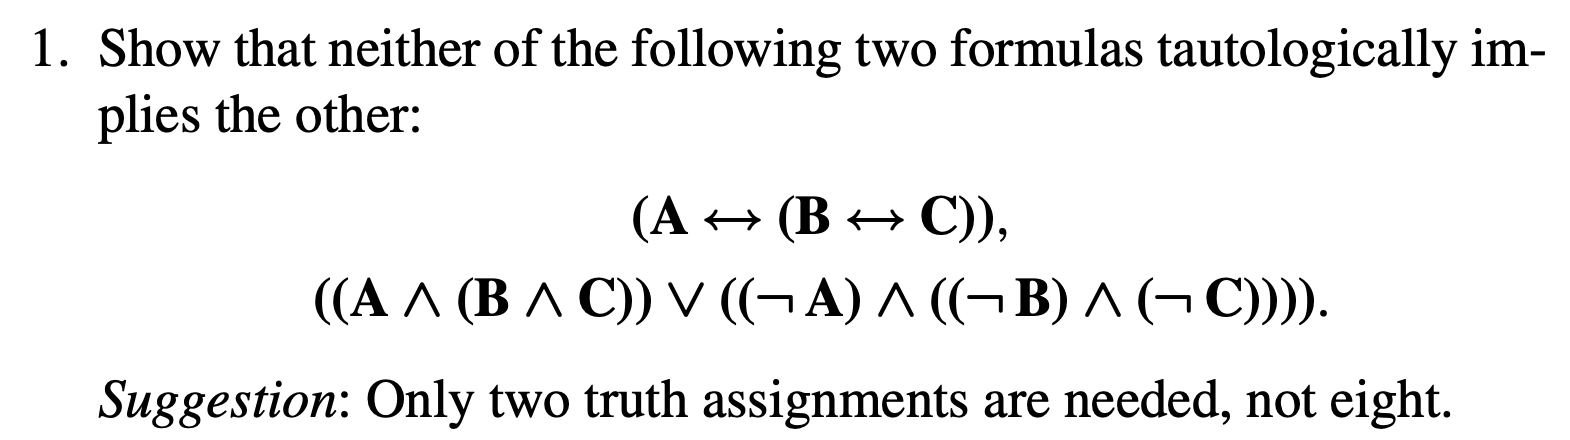
\includegraphics[width=400pt]{img/logic--berkeley-125a--homework-1-1a40.png}

\begin{definition}
  A formular $\phi$ \defn{tautologically implies} (aka \defn{semantically implies}) a formula $\varphi$ if every truth assignment that
  satisfies $\phi$ also satisfies $\varphi$.
\end{definition}

\begin{proof}
  With the truth assignment $(0, 0, 0)$ the RHS is true yet the LHS is false. Therefore there is no semantic
  implication in the forwards direction.

  With the truth assignment $(1, 0, 0)$ the LHS is true yet the RHS is false. Therefore there is no semantic
  implication in the reverse direction.

  \begin{table}[h!]
    \centering
    \begin{tabular}{|c|c|c|c|c|c|c|c|}
      A & B & C
      & $B \lequiv C$
      & A $\lequiv (B \lequiv C)$
      & $A \land (B \land C)$
      & $\lnot A \land (\lnot B \land \lnot C)$
      & $(A \land (B \land C)) \lor (\lnot A \land (\lnot B \land \lnot C))$\\
      \hline
      1 & 1 & 1 & 1&      1               &          1          &              0                 &  1    \\
      1 & 1 & 0 & 0&      0               &          0          &              0                 &  0    \\
      1 & 0 & 1 & 0&      0               &          0          &              0                 &  0    \\
      1 & 0 & 0 & 1&      1               &          0          &              0                 &  0    \\
      0 & 1 & 1 & 1&      0               &          0          &              0                 &  0   \\
      0 & 1 & 0 & 0&      1               &          0          &              0                 &  0    \\
      0 & 0 & 1 & 0&      1               &          0          &              0                 &  0    \\
      0 & 0 & 0 & 1&      0               &          0          &              1                 &  1    \\
    \end{tabular}
  \end{table}

\end{proof}



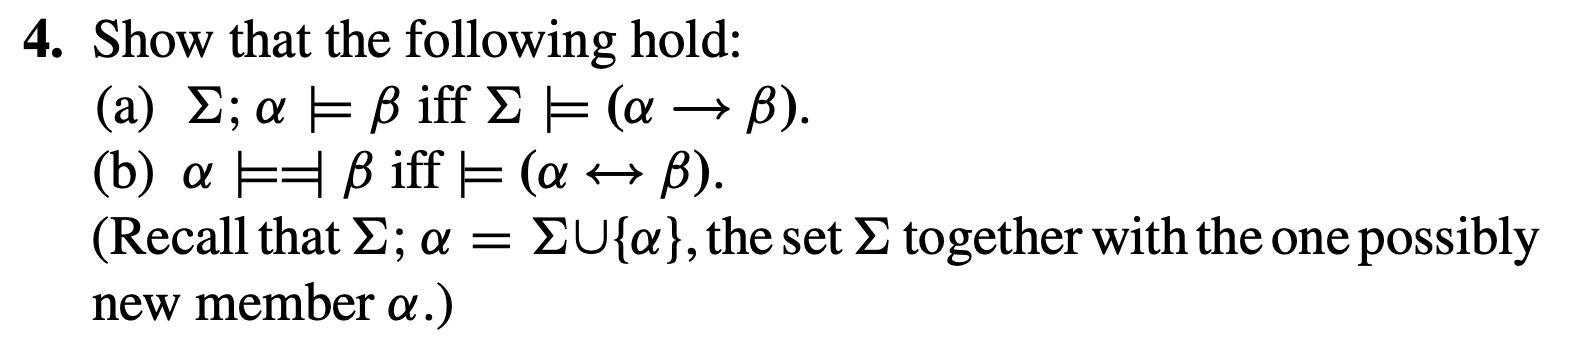
\includegraphics[width=400pt]{img/logic--berkeley-125a--homework-1-346f.png}



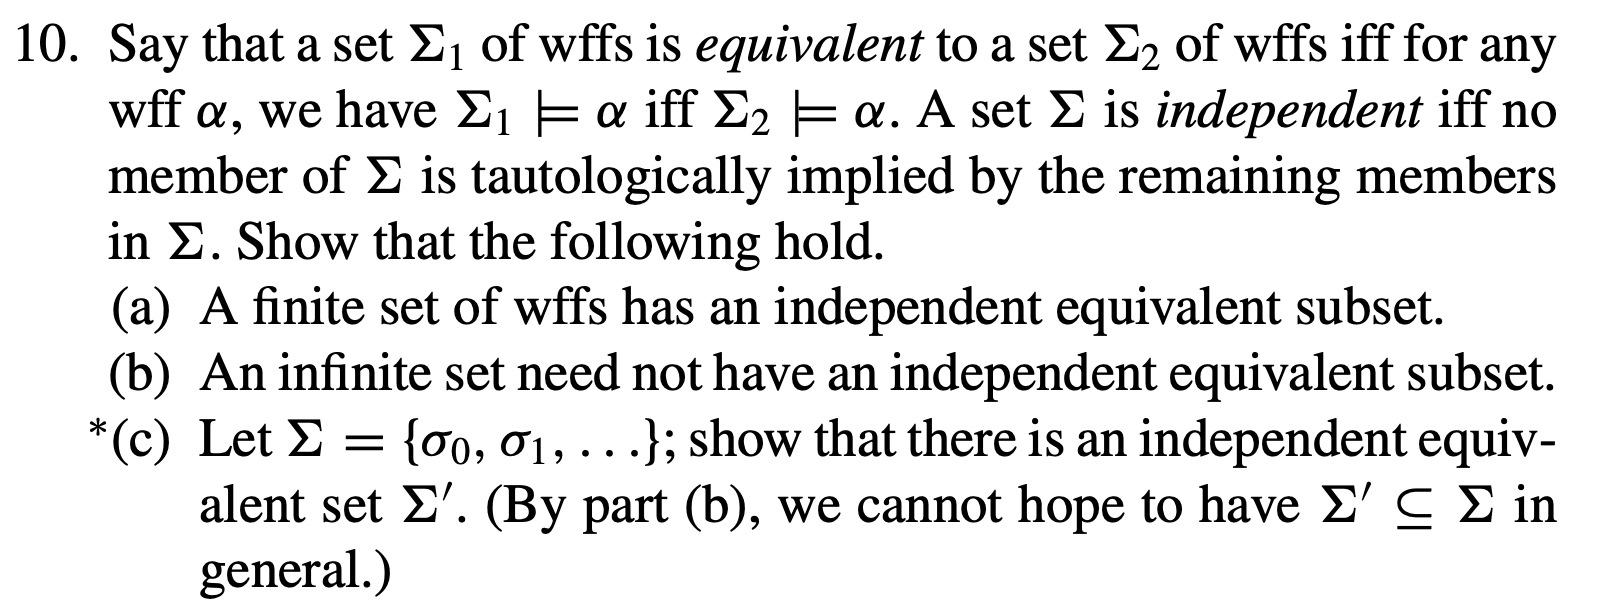
\includegraphics[width=400pt]{img/logic--berkeley-125a--homework-1-1b3d.png}



\includegraphics[width=400pt]{img/logic--berkeley-125a--homework-1-079f.png}

\includegraphics[width=400pt]{img/logic--berkeley-125a--homework-1-8256.png}


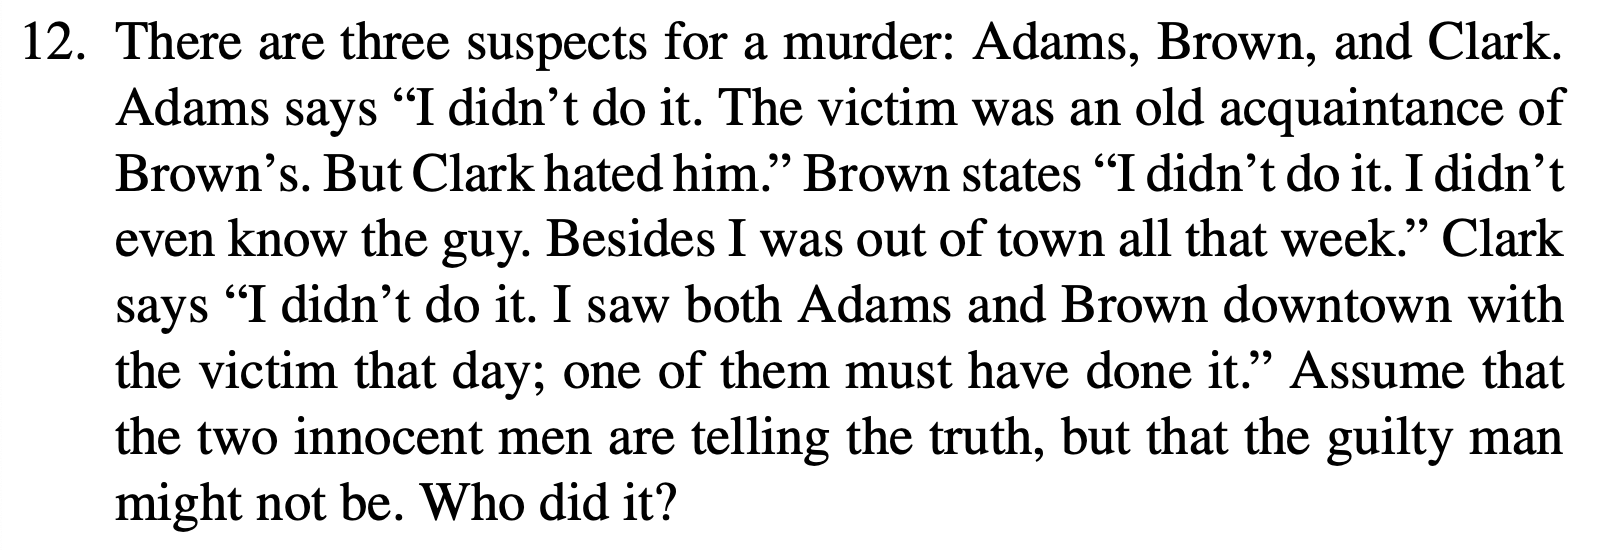
\includegraphics[width=400pt]{img/logic--berkeley-125a--homework-1-2358.png}


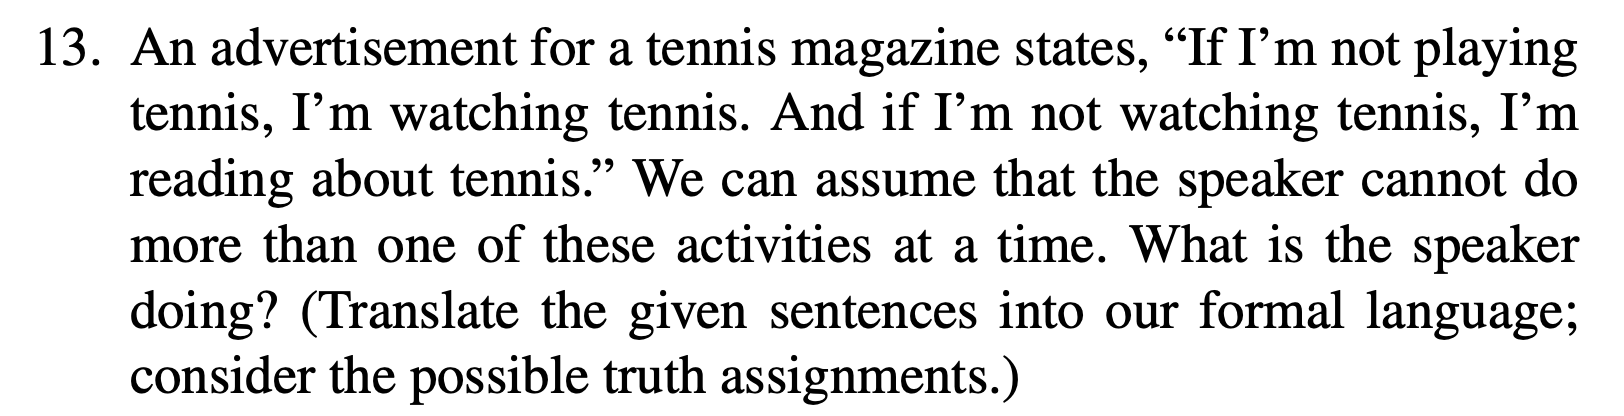
\includegraphics[width=400pt]{img/logic--berkeley-125a--homework-1-526e.png}

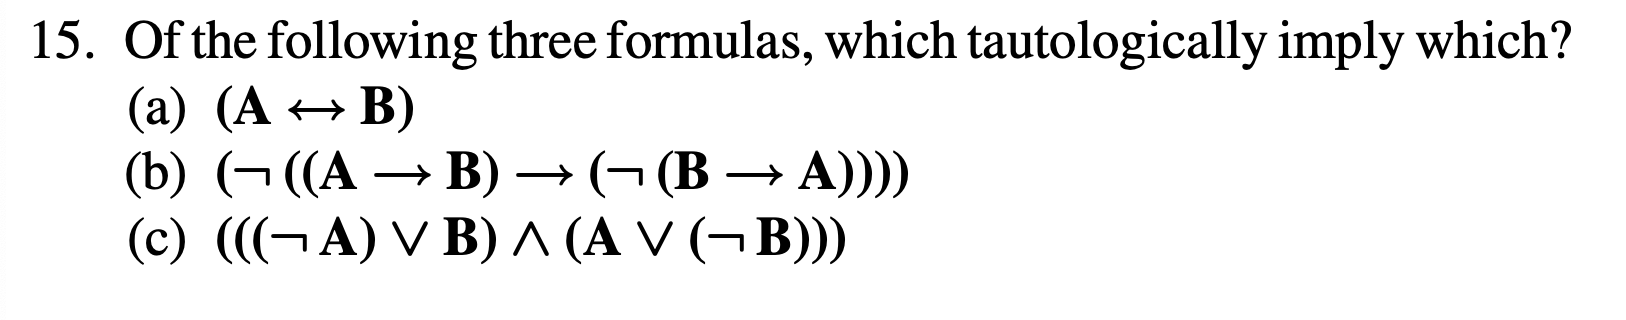
\includegraphics[width=400pt]{img/logic--berkeley-125a--homework-1-a71f.png}
